%%
%% This is file `sample-authordraft.tex',
%% generated with the docstrip utility.
%%
%% The original source files were:
%%
%% samples.dtx  (with options: `authordraft')
%% 
%% IMPORTANT NOTICE:
%% 
%% For the copyright see the source file.
%% 
%% Any modified versions of this file must be renamed
%% with new filenames distinct from sample-authordraft.tex.
%% 
%% For distribution of the original source see the terms
%% for copying and modification in the file samples.dtx.
%% 
%% This generated file may be distributed as long as the
%% original source files, as listed above, are part of the
%% same distribution. (The sources need not necessarily be
%% in the same archive or directory.)
%%
%% The first command in your LaTeX source must be the \documentclass command.
% \documentclass[sigconf,authordraft]{acmart}
\documentclass[10pt,sigconf,letterpaper,anonymous]{acmart}

\usepackage{algorithmic}
\usepackage{algorithm}

%%
%% \BibTeX command to typeset BibTeX logo in the docs
\AtBeginDocument{%
  \providecommand\BibTeX{{%
    \normalfont B\kern-0.5em{\scshape i\kern-0.25em b}\kern-0.8em\TeX}}}

%% Rights management information.  This information is sent to you
%% when you complete the rights form.  These commands have SAMPLE
%% values in them; it is your responsibility as an author to replace
%% the commands and values with those provided to you when you
%% complete the rights form.
\setcopyright{acmcopyright}
\copyrightyear{2019}
\acmYear{2019}
% \acmDOI{10.1145/1122445.1122456}

%% These commands are for a PROCEEDINGS abstract or paper.
\acmConference[Woodstock '18]{Woodstock '18: ACM Symposium on Neural
  Gaze Detection}{June 03--05, 2018}{Woodstock, NY}
\acmBooktitle{Woodstock '18: ACM Symposium on Neural Gaze Detection,
  June 03--05, 2018, Woodstock, NY}
\acmPrice{15.00}
\acmISBN{978-1-4503-9999-9/18/06}


%%
%% Submission ID.
%% Use this when submitting an article to a sponsored event. You'll
%% receive a unique submission ID from the organizers
%% of the event, and this ID should be used as the parameter to this command.
%%\acmSubmissionID{123-A56-BU3}

%%
%% The majority of ACM publications use numbered citations and
%% references.  The command \citestyle{authoryear} switches to the
%% "author year" style.
%%
%% If you are preparing content for an event
%% sponsored by ACM SIGGRAPH, you must use the "author year" style of
%% citations and references.
%% Uncommenting
%% the next command will enable that style.
%%\citestyle{acmauthoryear}

%%
%% end of the preamble, start of the body of the document source.
\begin{document}

%%
%% The "title" command has an optional parameter,
%% allowing the author to define a "short title" to be used in page headers.
\title{Bandwidth Reservation in Deterministic Networks (Detnet)}

%%
%% The "author" command and its associated commands are used to define
%% the authors and their affiliations.
%% Of note is the shared affiliation of the first two authors, and the
%% "authornote" and "authornotemark" commands
%% used to denote shared contribution to the research.
\author{Vamsi Addanki}
\email{f2013790@goa.bits-pilani.ac.in}
\affiliation{%
  \institution{Telecom-Paristech}
  \streetaddress{23 Avenue d'italie}
  \city{Paris}
  \state{France}
  \postcode{75013}
}

\author{Luigi Iannone}
\email{luigi.iannone@telecom-paristech.fr}
\affiliation{%
  \institution{Telecom-Paristech}
  \streetaddress{23 Avenue d'italie}
  \city{Paris}
  \state{France}
  \postcode{75013}
}


%%
%% By default, the full list of authors will be used in the page
%% headers. Often, this list is too long, and will overlap
%% other information printed in the page headers. This command allows
%% the author to define a more concise list
%% of authors' names for this purpose.
\renewcommand{\shortauthors}{addanki and luigi, et al.}

%%
%% The abstract is a short summary of the work to be presented in the
%% article.
\begin{abstract}
 Packet delivery in the Internet works as a best effort service. It has no guarantees. The end-to-end latency, jitter and packet-loss probability have no fixed bounds. In contrast, deterministic networks which is of interest in special cases, aims at guaranteed bounded latency and zero packet loss for priority set of flows. The techniques adopted in such kind of networks such as bandwidth-reservation and packet-replication are well described in the RFC. In this paper, we discuss the selection of algorithms for each technique and show the comparison between deterministic networks vs best effort service by simulations using ns-3. We mainly focus on bandwidth reservation part of deterministic networks. Although bandwidth is reserved for priority flows, there is still some unreserved bandwidth for non-priority flows. We aim at zero congestion loss for priority flows by bandwidth reservation, and fair usage of unreserved and/or total unused bandwidth for non-priority flows. In contrary to the idea of increasing number of buffers to reduce the probability of packet loss, we show that the algorithm we adopt for Deterministic networks can achieve zero packet loss with the same existing number of buffers (only one shared buffer for all flows in our experiments). 
\end{abstract}

%%
%% The code below is generated by the tool at http://dl.acm.org/ccs.cfm.
%% Please copy and paste the code instead of the example below.
%%
\begin{CCSXML}
<ccs2012>
 <concept>
  <concept_id>10010520.10010553.10010562</concept_id>
  <concept_desc>Computer systems organization~Embedded systems</concept_desc>
  <concept_significance>500</concept_significance>
 </concept>
 <concept>
  <concept_id>10010520.10010575.10010755</concept_id>
  <concept_desc>Computer systems organization~Redundancy</concept_desc>
  <concept_significance>300</concept_significance>
 </concept>
 <concept>
  <concept_id>10010520.10010553.10010554</concept_id>
  <concept_desc>Computer systems organization~Robotics</concept_desc>
  <concept_significance>100</concept_significance>
 </concept>
 <concept>
  <concept_id>10003033.10003083.10003095</concept_id>
  <concept_desc>Networks~Network reliability</concept_desc>
  <concept_significance>100</concept_significance>
 </concept>
</ccs2012>
\end{CCSXML}

\ccsdesc[500]{Computer systems organization~Embedded systems}
\ccsdesc[300]{Computer systems organization~Redundancy}
\ccsdesc{Computer systems organization~Robotics}
\ccsdesc[100]{Networks~Network reliability}

%%
%% Keywords. The author(s) should pick words that accurately describe
%% the work being presented. Separate the keywords with commas.
\keywords{datasets, neural networks, gaze detection, text tagging}

%% A "teaser" image appears between the author and affiliation
%% information and the body of the document, and typically spans the
%% page.
% \begin{teaserfigure}
%   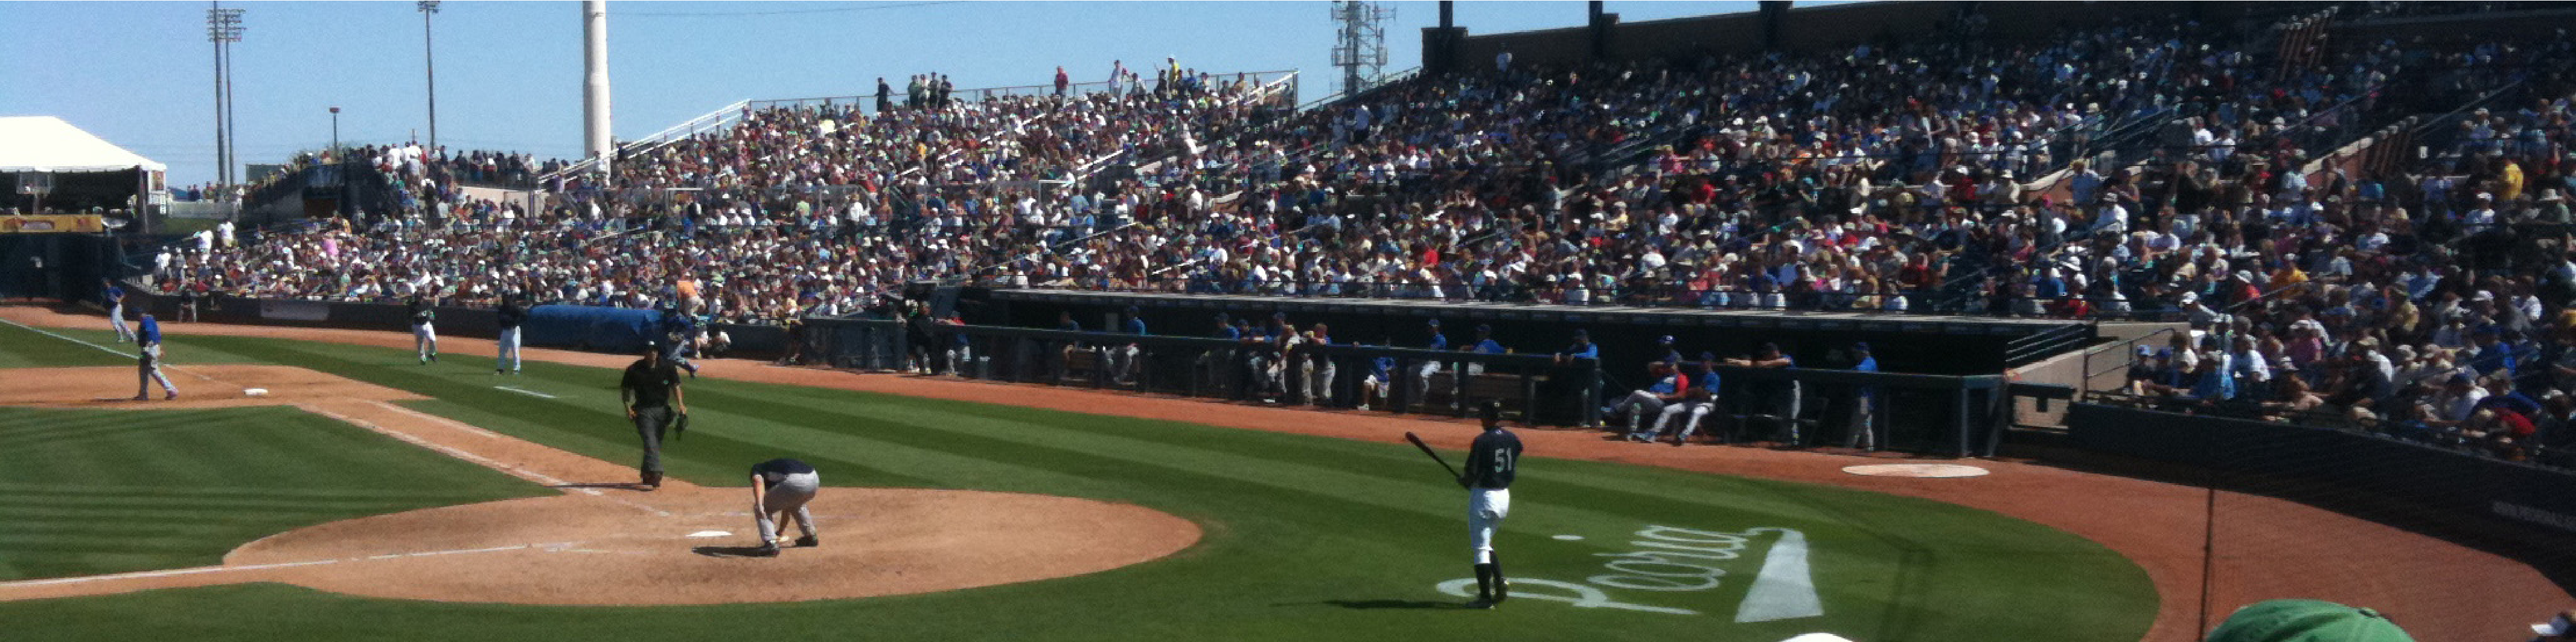
\includegraphics[width=\textwidth]{sampleteaser}
%   \caption{Seattle Mariners at Spring Training, 2010.}
%   \Description{Enjoying the baseball game from the third-base
%   seats. Ichiro Suzuki preparing to bat.}
%   \label{fig:teaser}
% \end{teaserfigure}

%%
%% This command processes the author and affiliation and title
%% information and builds the first part of the formatted document.
\maketitle

\section{Introduction}
Deterministic networks is part of time sensitive networking. In this type of networks, a bounded latency and zero congestion loss is guaranteed to a set of priority flows. This can be achieved by mechanisms such as explicit bandwidth reservation, packet replication \cite{detnetrfc}. The transmitter on the other end is also limited to a specific bandwidth. Although the type of mechanisms to be used in such networks are well described in the RFC and white-papers, there is no study in the literature about the possible algorithms that can be used in Deterministic Networks. \cite{detnetrfc}, \cite{detnetwhitepaper} suggest that increase in number of allocated buffers and explicit bandwidth reservation reduce the probability of packet-loss close to zero. 

Limiting the transmitter to a specific bandwidth and explicitly allocating resources in the network can be viewed as having virtually a separate link for each priority flow with a bandwidth equal to the reserved bandwidth. This leads to under-usage of bandwidth when the priority flows are inactive. In this paper, we propose an algorithm inspired from \cite{fairdroppaper}. The concept of virtual queues allows us to explicitly allocate resources to priority flows without increasing the number of real packet buffers. While the bandwidth is shared by priority and non-priority flows, we show that our algorithm optimizes the usage of unreserved and unused-reserved bandwidth by fairly sharing it among the non-priority flows. Our algorithm acts a dropper before en-queuing a packet in the queue.

Bandwidth sharing has always been a classical problem in networking. Numerous algorithms have been proposed for fair-sharing of bandwidth like FRED, CHOKe. In our specific case, we aim at virtual bandwidth reservation (meaning, guaranteed maximum bandwidth) for priority flows in combination with fair sharing of the remaining bandwidth among non-priority flows. This makes it very complex and difficult to implement and make use of any of the algorithms proposed in the literature.
In view of Deterministic Networking, our algorithm, inspired from X, eliminates the problem of increased number of packet buffers in the network and also eliminates the unused bandwidth problem by allowing the non-priority flows to use the bandwidth. The algorithm is also extremely simple to be implemented in software routers which are gaining popularity in the recent times.

In this paper, we use NS-3, an industry standard network simulator to implement our algorithm. We introduce a new queue-disc which implements our algorithm under the traffic-control module of ns-3. We show by simulations, per-flow bandwidth usage, latency profiles, jitter and queue length. We make comparison between a network with our proposed queue-disc, a network with simple fifo queues and a network with explicit bandwidth reservation. We show that our simple algorithm can be implemented easily on hardware or software to achieve the notion of explicit bandwidth-reservation for priority flows in deterministic networks.

In the following section we describe the essential components required for flow level bandwidth reservation. In sec 3 we present the algorithm and in sec 4 we describe in short, the implementation in ns-3 and present the results from simulations.

\section{Bandwidth reservation}

In the context of bandwidth sharing, numerous algorithms from literature like RED, CHOKE are stateless. This makes it difficult to achieve exact per-flow fair sharing of bandwidth. In a preliminary evaluation, we found that Fair-drop algorithm \cite{c} is stateful and achieves exact fair sharing of available bandwidth among concurrent flows. The concept of virtual queues introduced in this algorithm makes it easier for us to adopt some of the concepts into our algorithm to achieve per-flow bandwidth reservation and per-flow bandwidth sharing at the same time. The essential components of our algorithm are one global flow-table and two active-lists, one for each priority/non-priority set of flows. Fig. [\ref{fig:flowtable}] shows the structure of flow-table and active-list we use.

\subsection{Flow Table}
At the beginning, the flowtable is initialized with TABLESIZE rows and 1 column. Flows are classified based on rss hash value (HASH). RSS hash value is calculated by most of the hardware NICs in the recent times. So there is no overhead for the calculation of hash value. 

Algorithm [\ref{algo:flowclassification}] explains the flow classification. On packet arrival, HASH\%TABLESIZE is calculated, which gives the row index for the flow entry in the flow table. Then a linear search is applied in the row to find the flow entry for the current packet. If there is no entry for this flow yet, a new flow entry is created at the end of the row.
When a new entry is created, the entry is initialized the following values: packet-size, type (priority/non-priority), bandwidth reservation, last-arrival, virtual queue and threshold (related to algorithm).

The scalability of the flow-table comes from the fact that deterministic network is a small-scale network typically a local-area-network. Given this scenario, a good Hash function typically yields a widely spaced range of Hash values for IP address (2 fields of the 5-tuple) in same or adjacent subnets. So the scale of flow-table collisions possible for this kind of network is expected to be low.

\begin{algorithm}
\caption{\textbf{flow\_classify($pkt$)}}
\label {algo:flowclassification}
\begin{algorithmic}[1]
\STATE \textbf{Given:} queue item of the packet = pkt; TABLESIZE; flow\_table
\STATE hash = pkt.gethash;
\STATE mod = hash\%TABLESIZE;
\FOR{i in 0 to n entries in flow\_table[mod]}
\STATE flow\_entry=flow\_table[mod][i];
\IF {hash == flow\_entry.hash}
\STATE \textbf{return} flow\_entry;
\ENDIF
\ENDFOR
\STATE create a new flow table entry flow\_table[mod][n+1];
\STATE flow\_entry = flow\_table[mod][n+1];
\STATE flow\_entry.hash=hash
\STATE flow\_entry.vqueue=pkt.getSize();
\STATE flow\_entry.type=pkt.getType();
\STATE flow\_entry.last\_arrival=now();
\STATE flow\_entry.bwreq=pkt.Getbwreq();
\STATE flow\_entry.flow\_threshold=THRESHOLD;
\STATE \textbf{return} flow\_entry;
\end{algorithmic}
\end{algorithm}

\subsection{Active-list}
Active-list is simply a list of all flows which have their virtual queue greater than zero. On packet-arrival and flow-classifications, it's virtual queue is checked. If it is zero, the flow is added to active-list corresponding to the type of the flow.


\begin{figure}[ht]
	\begin{center}
		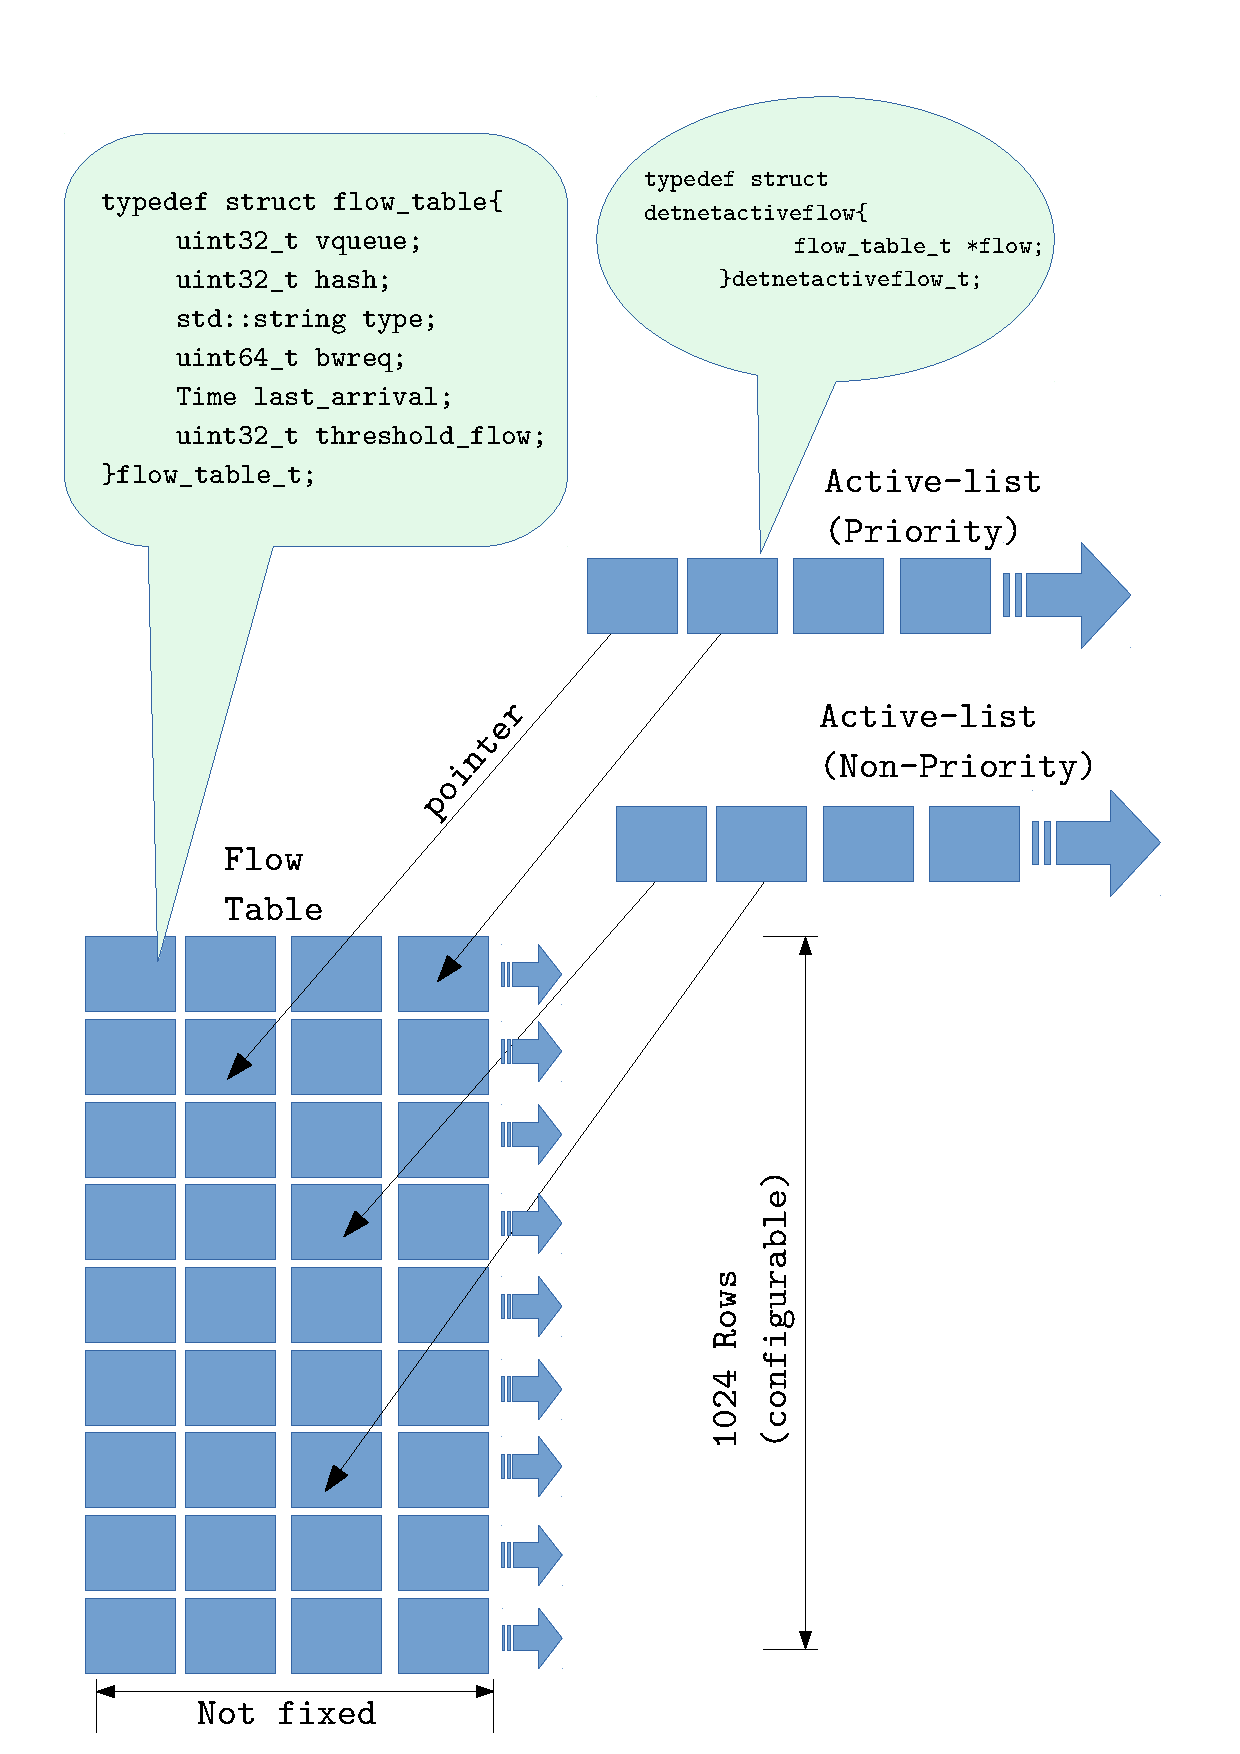
\includegraphics[width=0.50\textwidth]{figures/flowtable.pdf}
		\caption{Flow-table and active-list structures}\label{fig:flowtable}
	\end{center}
\end{figure}



\section{Algorithm}

Among the numerous concurrent flows, we have priority flows (PF) and non priority flows (N\_PF). In the context of deterministic networks, we need to reserve bandwidth for priority flows or guarantee a maximum bandwidth utilization for the flow. We achieve this by defining a maximum bandwidth utilization variable (bwreq) for each priority flow as shown in Fig. [\ref{fig:flowtable}]. As long as the incoming flow bandwidth is less than bwreq, we make sure that the flow experiences close to zero packet loss. The un-utilized bandwidth (independent of total reserved bandwidth) is fairly shared among all the concurrent non-priority flows. The algorithm consists of two stages.

\subsection {stage-1}
Stage-1 of the algorithm occurs at each packet arrival before en-queuing the packet in the output queue. The total available bandwidth (credit), is calculated by the difference between the arrival times of the current packet and the previous packet multiplied with the total output bandwidth. An additional credit type is also calculated for all the priority flows in the priority active-list. Priority-flow available bandwidth (priority-credit) calculated by the difference between the arrival times of the current packet and the last packet arrival of the corresponding priority flow multiplied with its reserved bandwidth. 
\begin{equation}
credit=(t_n - t_{n-1})*(BW_{output})\label{credit}
\end{equation}
\begin{equation}
priority\_credit_{pf}=(t_{npf}-t_{npf-1})*(BW_{reserved})\label{prioritycredit}
\end{equation}

First, the virtual queue of all the entries in the priority activelist are decremented by the priority credit corresponding to the priority flow. If the virtual queue is decremented to zero, the flow is removed from the activelist. Otherwise the flow's activelist position is changed to the end of the list. During this step, while decrementing the virtual queues of all active priority flows, the priority credit which is unused is added to ``remaining-credit'' cumulatively.

Then, the remaining-credit is added to credit and this is fairly divided among the entries of the activelist of non-priority flows. Similar to the previous step, if the flow under consideration in the loop reaches to zero size virtual queue, it is removed from activelist. Otherwise the flow's activelist position is changed to the end of the list.

\begin{algorithm}
\caption{\textbf{BW Reservation (Stage-1)}}
\label {algo:stage11}
\begin{algorithmic}[1]
\STATE \textbf{Given:} priority and non-priority activelists, flowtable;
\STATE $now$=time\_now();
\STATE $priority\_consumption$ = 0;
\IF{size of priority activelist $>$ 0}
\FOR{i in 0 to size of activelist}
\STATE $flow$ = get the first entry in activelist;
\STATE $\Delta t$ = $now$ - $flow.last\_arrival$;
\STATE $priority\_credit$ = $\Delta t$ * $flow.bwreq$;
\IF {$flow.vqueue$ $>$ $priority\_credit$}
\STATE $flow.vqueue$ -= $priority\_credit$;
\STATE $priority\_consumption$ += $priority\_credit$;
\STATE move the entry to the end of the activelist;
\ELSE 
\STATE $flow.vqueue$ = 0;
\STATE $priority\_consumption$ += $flow.vqueue$;
\STATE remove the entry from the activelist;
\ENDIF
\ENDFOR
\ENDIF
\end{algorithmic}
\end{algorithm}

\begin{algorithm}
\caption{\textbf{Remanining BW fair sharing (Stage-1)}}
\label {algo:stage12}
\begin{algorithmic}[1]
\STATE \textbf{Given:} priority and non-priority activelists, flowtable, variables from Algorithm \ref{algo:stage11};

\STATE $credit$ = $now$ - $Last Packet Arrival$;
\IF{$credit$ $>$ $priority\_consumption$ $\&\&$ size of non-priority activelist $>$ 0}

\STATE $remaining\_credit$ = $credit$ - $priority\_consumption$
\WHILE {$SizeofNon-PriorityActivelist$ $>$ 0 and $remaining\_credit$ $>$ 0}
\STATE $fairbw$ = $remaining\_credit$ / $sizeofActivelist$
\STATE $remaining\_credit$ = 0;
\FOR {each $flow$ in Activelist}
\IF {$flow.vqueue$ $>$ $fairbw$}
\STATE $flow.vqueue$ -= $fairbw$
\STATE move the entry to the end of the activelist;
\ELSE
\STATE $remaining\_credit$ += $fairbw$ - $flow.vqueue$;
\STATE $flow.vqueue$ = 0;
\STATE remove the entry from activelist;
\ENDIF
\ENDFOR
\ENDWHILE
\ENDIF

\end{algorithmic}
\end{algorithm}

\subsection {stage-2}

\begin{algorithm}
\caption{\textbf{On packet arrival (Stage-2)}}
\label {algo:stage2}
\begin{algorithmic}[1]
\STATE \textbf{Given:} packet's flow entry $flow$, $packet\_size$;
\IF {$flow.vqueue$ $>$ $THRESHOLD$}
\STATE drop();
\STATE exit();
\ELSE
\IF{$flow.vqueue$ == 0}
\STATE add the flow to the corresponding activelist by type.
\ENDIF
\STATE $flow.vqueue$ += $packet\_size$;
\STATE $flow.last\_arrival$ = now();
\ENDIF
\end{algorithmic}
\end{algorithm}


After stage-1, if the sum of current packet size and it's flow virtual queue is less than a THRESHOLD, the packet is enqueued in the output buffer and the packet size is added to it's virtual queue. Otherwise, the packet is dropped.
\\

By this, we make sure that the priority flows are always served first based on their reserved bandwidth and only then the non-priority flows are served. As a matter of fact, if the transmitter obeys the limit of reserved bandwidth, we observe close to zero packet loss for all priority flows. Thus we achieve a combination of bandwidth-reservation and bandwidth-fairsharing in deterministic networks.



\section{NS-3 Simulations}

\subsection{Implementation}
We introduced a new queue disc ``BW\_RESV'' under the traffic-control layer of ns-3. The algorithm is implemented in the en-queuing operation of this queue disc. We use On-off application of ns-3 as packet-generator. To simplify the configurations done by network administrators in the real world, we send a payload in each packet. The payload is of the format ``XXXXKbps Y''. Here X are 4 numeric digits for the reserved bandwidth/bitrate, Y is the type of flow where D corresponds to priority flow and O corresponds to non-priority flow (for example ``1000kbps D''). When a packet arrives at ``BW\_RESV'' queue disc for the first time, the packet payload is read to identify the type of the flow and it's bandwidth requirement. 

\subsection{Topology}
We use a simple network with 4 hosts and 2 routers. Two hosts are connected to each router and the two routers are connected to each 
other, as shown in Fig. [\ref{fig:topology}]. Host-1, Host-2 generate traffic and Host-3, Host-4 act as sink. All the links in the network are 30 Mbps except the link between the routers, which is 10 Mbps. The input link of Router-1 is configured high so that the output link becomes a bottleneck when there is a heavy traffic at the input. Router-1 is installed with either ``FIFO'' or ``BW\_RESV'' queue disc in the simulations.

% \begin{figure}[ht]
% 	\begin{center}
% 		\includegraphics[width=0.50\textwidth]{figures/topology.pdf}
% 		\caption{Topology}\label{fig:topology}
% 	\end{center}
% \end{figure}
\subsection{Simulations}
We generate 12 flows out of which 10 flows are priority flows and 2 flows are non-priority flows. The priority flows are configured with bandwidth reservation of 100Kbps, 200Kbps and so on upto 1Mbps for priority flow 1-10. All the priority flows are generated at 1000Kbps bitrate and non-priority flows are generated at 8000Kbps. With this traffic, we have no congestion in any of the links, except the 10Mbps link, which is the output of Router-1. Non-priority flow-1 and flow-2 start at t=0 and t=2 respectively. Priority flows start at t=1, t=3, t=4, t=5 and so on, one flow at each second. We run simulations using this traffic configuration with our ``BW\_RESV'' and ``FIFO'' queues to make a comparison and show that we can achieve bandwidth reservation and sharing at the same time using same resources.

\begin{figure}[ht]
	\begin{center}
		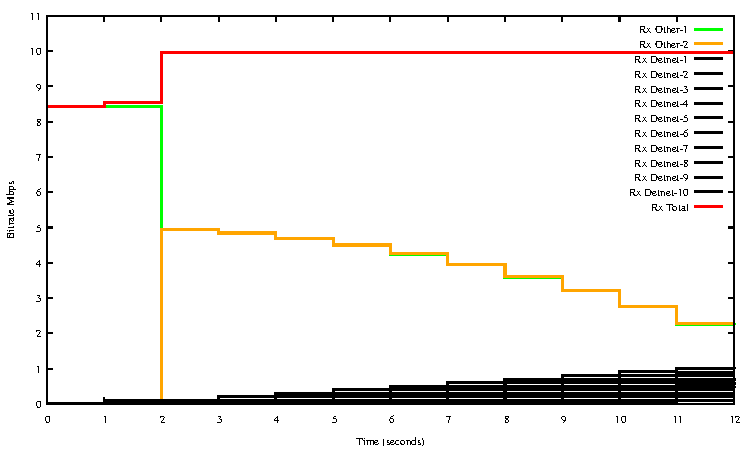
\includegraphics[width=0.50\textwidth]{plots/rx_detnet.pdf}
		\caption{Output rate per flow when bwresev queue is activated on the router with bottleneck link.}\label{fig:rx_detnet}
	\end{center}
\end{figure}
\begin{figure}[ht]
	\begin{center}
		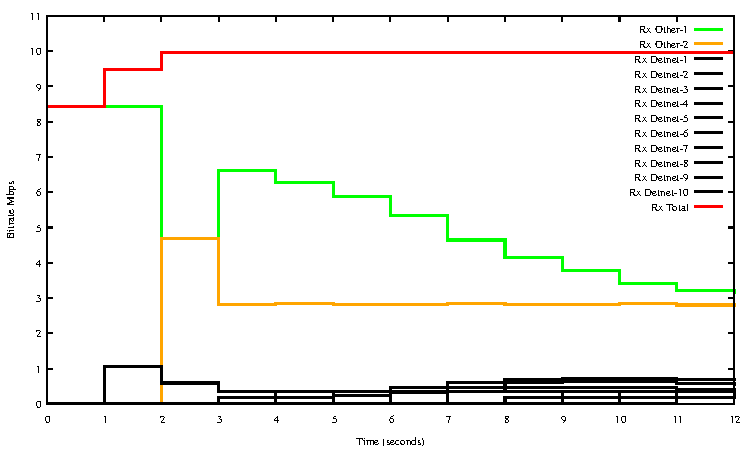
\includegraphics[width=0.50\textwidth]{plots/rx_fifo.pdf}
		\caption{Output rate per flow with fifo queues at the output of the router with bottleneck link.}\label{fig:rx_fifo}
	\end{center}
\end{figure}

\subsubsection{Throughput}
Throughput of flows at the output of Router-1 (with bottleneck link) is measured. From Fig. [\ref{fig:rx_detnet}], we can see that between t=0 and t=2, there is no congestion and no flow experiences drops. Starting from t=2, when the non-priority flow-2 starts, we see that priority flow-1 is given exactly the configured bandwidth reservation i.e 100Kbps for flow-1 and the remaining bandwidth is shared by the two non-priority flows. The same pattern continues in the graph. When an additional priority flow is introduced, the remaining bandwidth reduces and it is fairly shared by the two non-priority flows. In this case, the difference between flow's input and output throughput is entirely due to dropping of packets by the algorithm based on the reservation and sharing configurations. 

Fig. [\ref{fig:rx_fifo}] shows a simulation with Router-1 configured with ``FIFO'' queue at the output. This scenario can be compared to best-effort service. We see that there is specific pattern in how the output bandwidth is shared. Most importantly, the priority flows don't always get the reserved bandwidth at the output due to the excessive usage of bandwidth by non-priority and other priority flows.

\begin{figure}[ht]
	\begin{center}
		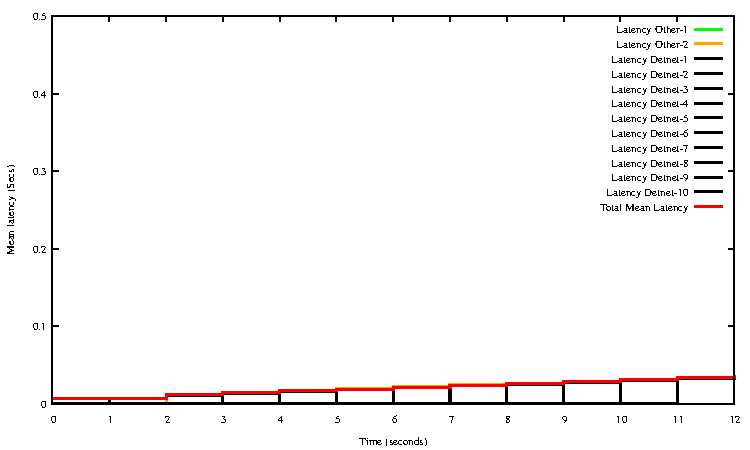
\includegraphics[width=0.50\textwidth]{plots/delay_detnet.pdf}
		\caption{Mean end-to-end latency when bw\_resv queue is installed}\label{fig:delay_detnet}
	\end{center}
\end{figure}
\begin{figure}[ht]
	\begin{center}
		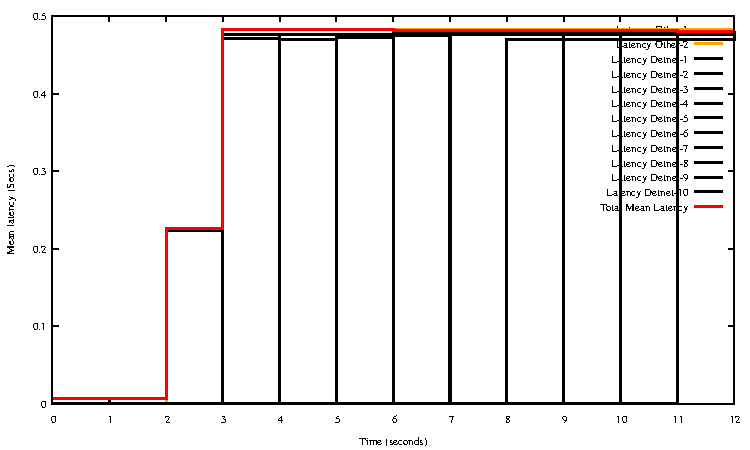
\includegraphics[width=0.50\textwidth]{plots/delay_fifo.pdf}
		\caption{Mean end-to-end latency with fifo queues}\label{fig:delay_fifo}
	\end{center}
\end{figure}

\subsubsection{Mean end-to-end Delay}
The mean end-to-end Delay is measured by simulations using flow-monitor module of ns-3. Fig. [\ref{fig:delay_fifo}] show a simulation with ``FIFO'' queues at Router's output. We see that the mean-delay stays very low until the queue is saturated and reaches a maximum when the queue is saturated. 

Fig. [\ref{fig:delay_detnet}] shows as simulation with ``BW\_RESV'' queue at Router's output. We see that the mean-delay is relatively very low and almost constant. Although, there is a small constant incremental value when the number of flows increase. This constant incremental value can be the overhead of measurement or the per-flow overhead of algorithm or a combination of both. It becomes extremely complex to isolate the cause since measuring time also consumes time. 

The most-important aspect of deterministic networks is bounded latency. We can clearly see from simulations that our algorithm can be configured properly to achieve a specific bounded latency.

\begin{figure}[ht]
	\begin{center}
		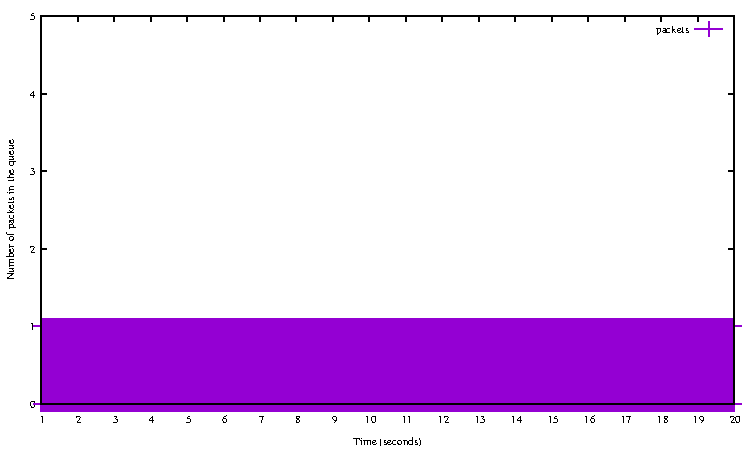
\includegraphics[width=0.50\textwidth]{plots/pkt_detnet.pdf}
		\caption{Mean Queue length of bw\_resv queue installed at the output of router-1}\label{fig:pkt_detnet}
	\end{center}
\end{figure}
\begin{figure}[ht]
	\begin{center}
		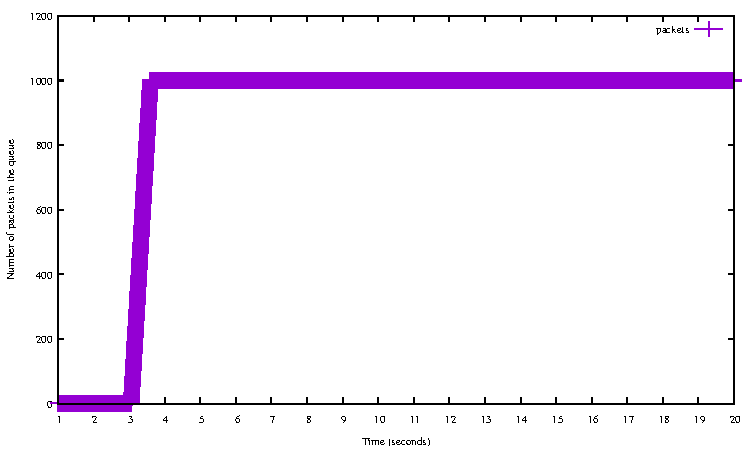
\includegraphics[width=0.50\textwidth]{plots/pkt_fifo.pdf}
		\caption{Mean Queue length of fifo queue installed at the output of router-1}\label{fig:pkt_fifo}
	\end{center}
\end{figure}

\subsubsection{Queue length}

We also measured the number of packets in the output queue of Router-1 at each packet arrival. We see that, in the case of ``FIFO'' queue from Fig. [\ref{fig:pkt_fifo}], the number of packets in the queue is close to zero until saturation, and starting from t=2, the queue length slowly reaches to full capacity and starts to drop packets. The increase in the queue length is one reason why the mean-delay of packets reaches a maximum due to the mean waiting-time in the queue.

We avoid this problem by making drop decisions at each packet arrival to avoid congestion in the output queue. This is done while ensuring the bandwidth reservation and sharing configurations. As a result, we see that the queue length stays close to zero.

\subsubsection{Packet Loss}
In this part, we run experiments with 12 flows consisting of 10 priority flows and 2 non-priority flows. All the priority flows transmit at 1Mbps with 1.1Mbps reservation and the non-priority flows transmit at 8Mbps. Each flow starts to transmit at times exactly same as in the previous experiments. (Non-priority-1 at t=0; Priority-1 at t=1; Non-priority-2 at t=2 and so on). When all the flows are in progress, they intersect at Router-1 with one output link of 12Mbps. As we can notice immediately, the output link is in an overload scenario. In this scenrio, we run experiments to check the overall packet loss experienced by the flows during the whole experiment. We can see from Fig. [\ref{fig:loss}] that the priority flows have an exact zero packet loss as expected since they all have a reservation of 1.1Mbps and transmit at lower rate. We can also see that there is a heavy packet loss with ``FIFO'' queues. 

\begin{figure}[ht]
	\begin{center}
		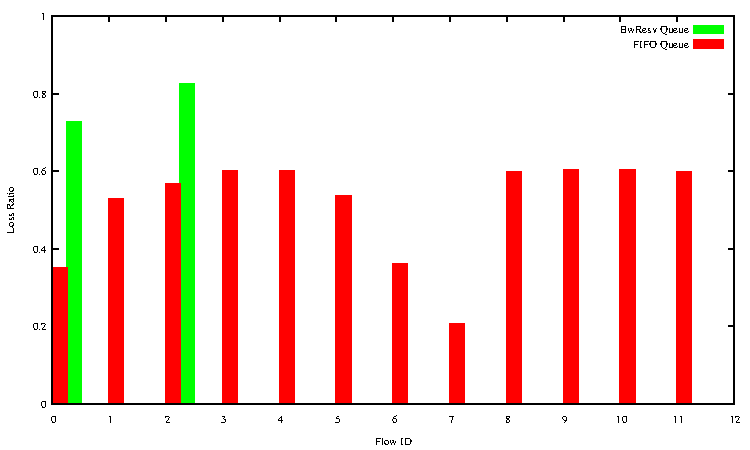
\includegraphics[width=0.50\textwidth]{plots/loss.pdf}
		\caption{Overall packet loss}\label{fig:loss}
	\end{center}
\end{figure}

\section {Conclusions}

\section{Acknowledgments}

Identification of funding sources and other support, and thanks to
individuals and groups that assisted in the research and the
preparation of the work should be included in an acknowledgment
section, which is placed just before the reference section in your
document.

This section has a special environment:
\begin{verbatim}
  \begin{acks}
  ...
  \end{acks}
\end{verbatim}
so that the information contained therein can be more easily collected
during the article metadata extraction phase, and to ensure
consistency in the spelling of the section heading.

Authors should not prepare this section as a numbered or unnumbered {\verb|\section|}; please use the ``{\verb|acks|}'' environment.

\section{Appendices}

If your work needs an appendix, add it before the
``\verb|\end{document}|'' command at the conclusion of your source
document.

Start the appendix with the ``\verb|appendix|'' command:
\begin{verbatim}
  \appendix
\end{verbatim}
and note that in the appendix, sections are lettered, not
numbered. This document has two appendices, demonstrating the section
and subsection identification method.

\section{SIGCHI Extended Abstracts}

The ``\verb|sigchi-a|'' template style (available only in \LaTeX\ and
not in Word) produces a landscape-orientation formatted article, with
a wide left margin. Three environments are available for use with the
``\verb|sigchi-a|'' template style, and produce formatted output in
the margin:
\begin{itemize}
\item {\verb|sidebar|}:  Place formatted text in the margin.
\item {\verb|marginfigure|}: Place a figure in the margin.
\item {\verb|margintable|}: Place a table in the margin.
\end{itemize}

%%
%% The acknowledgments section is defined using the "acks" environment
%% (and NOT an unnumbered section). This ensures the proper
%% identification of the section in the article metadata, and the
%% consistent spelling of the heading.
\begin{acks}
To Robert, for the bagels and explaining CMYK and color spaces.
\end{acks}

%%
%% The next two lines define the bibliography style to be used, and
%% the bibliography file.
\bibliographystyle{ACM-Reference-Format}
\bibliography{sample-base}

%%
%% If your work has an appendix, this is the place to put it.
\appendix

\section{Research Methods}

\subsection{Part One}

Lorem ipsum dolor sit amet, consectetur adipiscing elit. Morbi
malesuada, quam in pulvinar varius, metus nunc fermentum urna, id
sollicitudin purus odio sit amet enim. Aliquam ullamcorper eu ipsum
vel mollis. Curabitur quis dictum nisl. Phasellus vel semper risus, et
lacinia dolor. Integer ultricies commodo sem nec semper.

\subsection{Part Two}

Etiam commodo feugiat nisl pulvinar pellentesque. Etiam auctor sodales
ligula, non varius nibh pulvinar semper. Suspendisse nec lectus non
ipsum convallis congue hendrerit vitae sapien. Donec at laoreet
eros. Vivamus non purus placerat, scelerisque diam eu, cursus
ante. Etiam aliquam tortor auctor efficitur mattis.

\section{Online Resources}

Nam id fermentum dui. Suspendisse sagittis tortor a nulla mollis, in
pulvinar ex pretium. Sed interdum orci quis metus euismod, et sagittis
enim maximus. Vestibulum gravida massa ut felis suscipit
congue. Quisque mattis elit a risus ultrices commodo venenatis eget
dui. Etiam sagittis eleifend elementum.

Nam interdum magna at lectus dignissim, ac dignissim lorem
rhoncus. Maecenas eu arcu ac neque placerat aliquam. Nunc pulvinar
massa et mattis lacinia.

\end{document}
\endinput
%%
%% End of file `sample-authordraft.tex'.
